\chapter{Sistemas CAOS para planificaci\'on preoperatoria}

%%%%%%%%%%%%%%%%%%%%%%%%%%%%%%%%%%%%%%%%%%%%%%%%%%%
\section{Planificaci\'on preoperatoria}

La planificaci\'on preoperatoria o planificaci\'on prequir\'urgica es una disciplina sumamente importante que debe ser realizada por todos los cirujanos ortop\'edicos como requisito indispensable para llevar a cabo un determinado procedimiento quir\'urgico con excelentes resultados.

\begin{quote}
\textit{
	El tiempo que el cirujano ortopedista dedique a efectuar una cuidadosa planificaci\'on preoperatoria tiene una importancia decisiva y a menudo determina el \'exito o fracaso de una operaci\'on
	}
\end{quote}
\begin{center} \footnotesize \textit{Joseph Schatzker. Tratamiento Quir\'{u}rgico de las fracturas \cite{SCHA98}}. \end{center}

Como se describe en \cite{RUEDI03}, la planificaci\'on preoperatoria ortop\'edica es un procedimiento indispensable que debe realizarse previo a la intervenci\'on quir\'urgica y cuyos objetivos son: determinar el resultado final de la cirug\'ia y establecer la t\'actica quir\'urgica a seguir en el procedimiento quir\'urgico. 

La planificaci\'on preoperatoria para una cirug\'ia plantea la realizaci\'on de calcos preoperatorios, como se muestra en la Figura \ref{fig:planificacion}. Los calcos permiten entender la complejidad de la fractura, la forma de reducci\'on de la misma, las acciones a seguir para la reducci\'on y la elecci\'on del implante necesario.
\begin{figure}[htbp]
  \begin{center} \subfigure[]{\label{fig:plan1}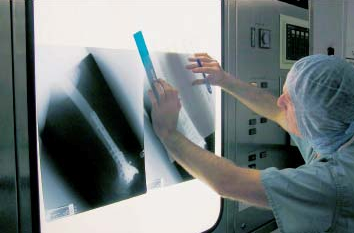
\includegraphics[width=0.45\columnwidth]{images/plan1.png}}  \subfigure[]{\label{fig:plan2}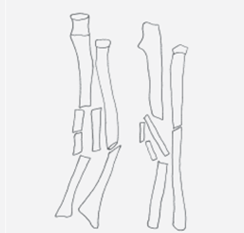
\includegraphics[width=0.31\columnwidth]{images/plan2.png}}   
  \end{center}
  \caption{Procedimiento manual para la creaci\'on de un calco preoperatorio. (a) Creaci\'on del calco sobre un negatoscopio (b) Calco obtenido}
  \label{fig:planificacion}
\end{figure}

En ciertos procedimientos quir\'urgicos, la planificaci\'on preoperatoria es parte integral de una cirug\'ia. Un ejemplo de ello, se muestra en \cite{EGGLI98,BENE03} donde se aplica planificaci\'on preoperatoria para la colocaci\'on de una pr\'otesis de cadera. Antes de la operaci\'on, es importante conocer ciertos factores previos: tipo y tama\~no de la pr\'otesis, posici\'on y orientaci\'on correcta de los implantes, tama\~no del acet\'abulo y del hueso. Al mismo tiempo, esta informaci\'on permite indicar los procedimientos a realizar durante la cirug\'ia y prever cualquier inconveniente. Estos procedimientos traen como resultado la reducci\'on del tiempo de cirug\'ia y garantizar, con un alto nivel de probabilidad, resultados satisfactorios.

Para tener \'exito en el resultado final de la cirug\'ia, R\"{u}edi et al. \cite{RUEDI03} sugieren que se deben realizar las siguientes acciones:
\begin{itemize}
	\item Tomar en cuenta los factores iniciales del contacto m\'edico-paciente.
	\item Crear una historia m\'edica completa.
	\item Realizar una evaluaci\'on preoperatoria.	
	\item Obtener radiograf\'ias para la planificaci\'on (preferiblemente sin inmovilizadores que obstaculicen la visi\'on adecuada).
	\item Si es necesario, realizar estudios especiales como CT, MRI, estudios de laboratorio, entre otros.
	\item Crear una planificaci\'on previa a la operaci\'on.
\end{itemize}

%%%%%%%%%%%%%%%%%%%%%%%%%%%%%%%%%%%%%%%%%%%%%%%%%%%
\subsection{Procedimiento para su realizaci\'on}

La planificaci\'on consiste en realizar un calco de los segmentos de fractura y del hueso, para as\'i tener una gu\'ia correspondiente a la anatom\'ia de la zona a tratar del paciente. De esta forma, el calco representa la herramienta de trabajo construida por el m\'edico traumat\'ologo para el proceso de fijaci\'on de la fractura (i.e. reconstrucci\'on del hueso). En una fractura, el equipo necesario para realizar las planificaciones se puede resumir en:
\begin{enumerate}
	\item Radiograf\'ias adecuadas: Estas radiograf�as opcionalmente incluyen el lado sano. El lado sano sirve para realizar comparaciones con respecto al lado fracturado, tomando en cuenta los factores de simetr\'ia del cuerpo humano.
	\item Papel para calcos: Es un papel especial (semitransparente) sobre el cual se dibujar\'a la imagen de los trazos de una fractura.
	\item Plantillas de los implantes: Conjunto de las posibles plantillas (\textit{templates}) de implantes (tornillos, clavos, placas, etc.) que puede necesitar una fractura. Cada fabricante de material quir\'urgico, e.g. tornillos, mantiene una librer\'ia de sus productos y \'estos son entregados a los Centros Hospitalarios. En la Figura \ref{fig:plantilla}, se puede observar una plantilla de tornillos.
	\item Goni\'ometro: Instrumento utilizado para medir valores angulares y rangos articulares. Existen m\'ultiples tipos de goni\'ometros, entre los que se destacan los goni\'ometros de dos brazos de eje com\'un y un cuadrante dividido en grados, que son los m\'as utilizados (ver Figura \ref{fig:goniometro}). Tambi\'en existen los goni\'ometros que se basan en la indicaci\'on permanente de la vertical; goni\'ometros que utilizan la desviaci\'on magn\'etica y goni\'ometros electr\'onicos. 
	\item L\'apices o marcadores de colores: Para poder realizar el trazo del calco.
	\item Negatoscopio con luz adecuada: Aparato constituido por una placa transl\'ucida colocada delante de una fuente luminosa, utilizada para examinar las radiograf\'ias. Es sobre este aparato donde son realizados los calcos.
\end{enumerate}

\begin{figure}[htbp]
	\centering
	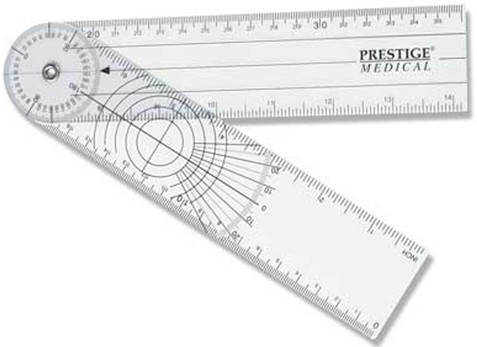
\includegraphics[width=.3\columnwidth]{images/goniometro.png}
	\caption{Goni\'ometro de dos brazos}
	\label{fig:goniometro}
\end{figure}

La elecci\'on del procedimiento quir\'urgico es determinada por las caracter\'isticas de la fractura u osteotom\'ia; hueso, regi\'on, tipo de trazo, desviaciones  angulares, rotaciones, acortamientos, n\'umero de fragmentos, tama\~no de los fragmentos  y las condiciones de los tejidos blandos.
 
La selecci\'on del implante o dispositivo adecuado para la osteos\'intesis debe incluir las acciones a seguir en la cirug\'ia, el abordaje quir\'urgico, el tipo de dispositivo, sus dimensiones, tipo de bloqueo (si lo requiere), dimensiones de los tornillos, orden de colocaci\'on, etc. Para las fracturas diafisiarias en las que est\'a indicada la fijaci\'on con un clavo intramedular bloqueado, se necesita una planificaci\'on gr\'afica preoperatoria poco detallada. Las variables que hay que determinar de acuerdo a lo expuesto en \cite{RUEDI03} son: la longitud y el di\'ametro del clavo intramedular, el fresado o no del canal endomedular y el tipo de bloqueo. La osteos\'intesis con placa requiere una planificaci\'on m\'as detallada, los puntos que deben considerarse son: la correcta longitud, alineaci\'on y rotaci\'on del hueso, el tipo y longitud de la placa, el n\'umero de tornillos y su funci\'on espec\'ifica (compresi\'on interfragmentaria o a trav\'es de la placa). Por \'ultimo, es importante destacar que la planificaci\'on preoperatoria de fracturas que comprometen las superficies articulares es m\'as exigente que las fracturas diafisiarias, puesto que requieren una reducci\'on anat\'omica exacta.

%%%%%%%%%%%%%%%%%%%%%%%%%%%%%%%%%%%%%%%%%%%%%%%%%%%
\subsection{Estrategia quir\'urgica}

En la estrategia quir\'urgica el cirujano ortopedista debe enumerar los pasos a seguir para el procedimiento con el fin de evitar distracciones y para el conocimiento del equipo quir\'urgico. De esta forma dicho equipo estar\'a mejor preparado para resolver los problemas que se puedan presentar. La estrategia quir\'urgica debe estar en el calco de la planificaci\'on preoperatoria, como se observa en la Figura \ref{fig:planificacion_completa}, y debe contener los siguientes puntos:

\begin{figure}[htb]
	\centering
	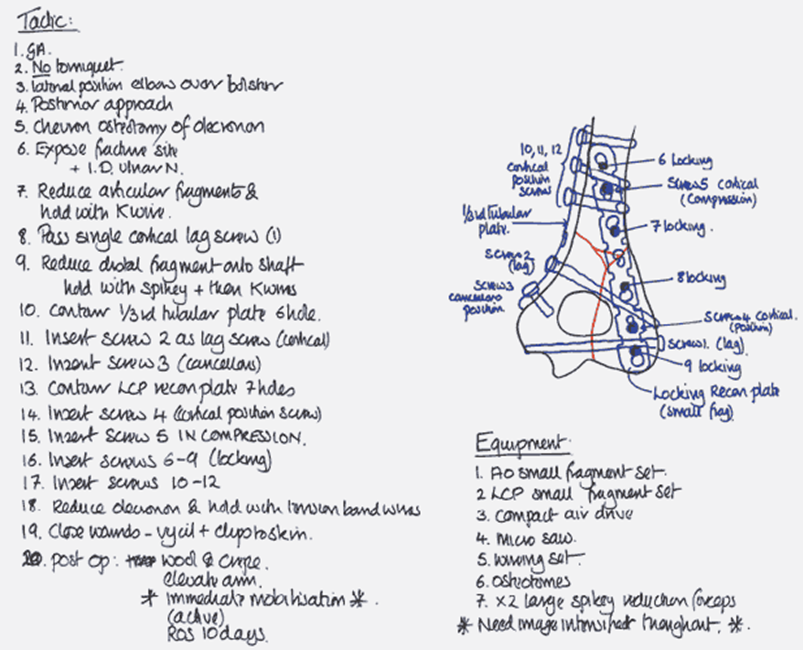
\includegraphics[width=.65\columnwidth]{images/planificacioncompleta.png}
	\caption{Calco de una fractura con la informaci\'on completa antes de la cirug\'ia}
	\label{fig:planificacion_completa}
\end{figure}

\begin{itemize}
	\item Paciente: Nombre y apellido, edad, uso de torniquete, posici\'on del paciente, uso de mesa radiol\'ucida.
	\item Procedimiento: Incluye los procedimientos a realizar durante la cirug\'ia, es decir, las acciones que el m\'edico va a realizar en la operaci\'on (e.g. selecci\'on del tipo de bistur\'i y n\'umero de incisiones, entre otros). Adem\'as incluye el tipo de reducci\'on a aplicar, implantes a emplear y la selecci\'on del equipo a utilizar para la colocaci\'on de implantes.
	\item Equipos Adicionales: Radiograf\'ias transoperatorias (radiograf\'ias tomadas durante la cirug\'ia) empleando un intensificador de im\'agenes, artroscopio, etc.
	\item Cuidados Postoperatorios: Uso de yesos, f\'erulas, pr\'otesis o vendajes en el postoperatorio inmediato.
\end{itemize}

Existen diversas t\'ecnicas de planificaci\'on preoperatoria, entre las que se destacan:
	\subparagraph{Superposici\'on Directa:} Utilizada en las planificaciones de fracturas diafisiarias. Se realiza el calco de los fragmentos fracturados en una proyecci\'on antero-posterior (AP), cada uno en hojas separadas. En otra hoja se traza una l\'inea recta (eje del hueso) y se colocan los fragmentos que son ensamblados para obtener el resultado final.
	\subparagraph{Superposici\'on utilizando la imagen del lado sano:} Se requiere la radiograf\'ia del lado sano y se procede a realizar el calco del lado fracturado tomando en cuenta los fragmentos y rotaciones, dibuj\'andolas en otro color. Luego se realiza la colocaci\'on de los fragmentos dibujados en la radiograf\'ia del lado sano para hacerlos coincidir. Otra forma es realizar la colocaci\'on de los fragmentos y posteriormente superponerla a la radiograf\'ia del lado sano para evaluar la colocaci\'on adecuada de los fragmentos, una vez que se tenga la reducci\'on de los mismos, se utilizan las plantillas de implantes y se completa el calco seg\'un la elecci\'on del cirujano ortopedista.
	\subparagraph{Superposici\'on utilizando los ejes fisiol\'ogicos:} Es una metodolog\'ia aplicable a aquellas fracturas periarticulares (fracturas producidas cercanas a una articulaci\'on), como es el caso de las fracturas supracond\'ileas de f\'emur las cuales son fracturas periarticulares de la porci\'on distal del f\'emur.
En una fractura distal de f\'emur se usa la plantilla para marcar los ejes anat\'omicos  y mec\'anicos del f\'emur y la tibia. Posterior a esto, se dibujan los fragmentos de la fractura y se superponen a la plantilla inicial, para hacer coincidir los ejes del f\'emur y la tibia y as\'i lograr la alineaci\'on de la rodilla. Una vez colocados todos los fragmentos reducidos se procede a la colocaci\'on del implante. \\

Particularmente, en este documento trataremos el caso de la planificaci\'on preoperatoria empleando la t\'ecnica de superposici\'on directa.

%%%%%%%%%%%%%%%%%%%%%%%%%%%%%%%%%%%%%%%%%%%%%%%%%%%
\section{Sistemas CAD}

Actualmente solo algunos cirujanos ortop\'edicos llevan a cabo dichas planificaciones, puesto que se requiere de material adicional y una inversi\'on considerable de tiempo para su realizaci\'on. Los sistemas de Diagn\'ostico Asistido por Computador (\textit{CAD - Computer Aided Diagnosis}) son excelentes herramientas para que los m\'edicos realicen diagn\'osticos m\'as acertados en un tiempo m\'as corto. Cada vez es m\'as frecuente la presencia de estos sistemas en el campo de la medicina, y particularmente existe un gran crecimiento en el \'area de Radiolog\'ia \cite{GIGE00}.

El concepto del CAD es amplio y general como herramienta de asistencia a los radi\'ologos, proporcionando una ``segunda opini\'on'' provista por el computador. Este aspecto, expuesto por Doi en \cite{DOI07}, es la principal diferencia con los sistemas de Diagn\'ostico Automatizado por Computador (\textit{Automated Computer Diagnosis}), los cuales son utilizados para diagnosticar autom\'aticamente cualquier condici\'on de salud-enfermedad (lesi\'on, s\'indrome, entidad nosol\'ogica, etc.). En un sistema CAD siempre el radi\'ologo tomar\'a la decisi\'on final.
 
Las investigaciones en el \'area del Diagn\'ostico Asistido por Computador \cite{HUANG07} se iniciaron en 1980 y han ido evolucionando gradualmente como una herramienta de apoyo cl\'inico. En el \'area de mamograf\'ia, los sistemas CAD se han convertido en una herramienta de rutina para la detecci\'on de c\'anceres de mama en muchos centros m\'edicos. Un gran n\'umero de sistemas CAD en Estados Unidos y Europa \cite{DOI07}, son utilizados para la detecci\'on temprana del c\'ancer de mama en las mamograf\'ias. Algunos sistemas CAD son utilizados para el registro de im\'agenes \cite{ZITO03} (\textit{image registration}), interacciones virtuales, visualizaci\'on, simulaci\'on y entrenamiento.

Por ejemplo, para los casos de entrenamiento y pr\'acticas educativas para estudiantes de medicina, Blyth et al. \cite{BLYT06} ofrecen una herramienta que simula escenarios virtuales a los futuros cirujanos. La necesidad de una simulaci\'on viene determinada por la complejidad de ciertas regiones del cuerpo humano, como la craniofacial o la regi\'on card\'iaca. Es muy importante que estructuras vitales del cuerpo humano no sean da\~nadas durante una operaci\'on, lo cual puede lograrse con el uso de sistemas de este tipo.

En el 2002, Bourquain et al. \cite{BOUR02} desarrollaron (\textit{HepaVision2}), una aplicaci\'on para la planificaci\'on preoperatoria de transplantes y cirug\'ias de h\'igado. \textit{HepaVision2} es una herramienta que trabaja con im\'agenes en formato DICOM \cite{REF_DICOM} (\textit{Digital Imaging and Communication in Medicine}) siendo capaz de realizar una segmentaci\'on del h\'igado empleando el algoritmo \textit{livewire} \cite{MORT95} de detecci\'on semiautom\'atica de bordes. Adem\'as, realiza el c\'alculo del volumen del h\'igado y las venas hep\'aticas que permiten determinar los tumores. Esta versi\'on del software trabaja sobre PCs basadas en \textit{Windows} y provee un m\'odulo de an\'alisis de riesgo de operaci\'on en el paciente a tratar.

%%%%%%%%%%%%%%%%%%%%%%%%%%%%%%%%%%%%%%%
\subsection{Cirug\'ia Ortop\'edica Asistida por Computador}

Diversos software de apoyo al cirujano para la reducci\'on de fracturas en extremidades inferiores son utilizados desde hace varios a\~nos, un ejemplo de ello se muestra en  \cite{TOCKUS98, NAKA24}. Los sistemas CAD de planificaci\'on preoperatoria de cirug\'ias del sistema muscoesquel\'etico, son conocidos como CAOS (\textit{Computer Aided Orthopaedic Surgery}) los cuales son foco de investigaci\'on en diversas partes del mundo \cite{BRAN99, LANG98, RADE98, MART00}.

Al realizar la planificaci\'on preoperatoria con \'estas herramientas, el proceso se torna m\'as preciso y repetible que los m\'etodos convencionales/tradicionales, como el uso de plantillas mostrado en la Figura \ref{fig:plantilla}. 
\begin{figure}[htb]
	\centering
	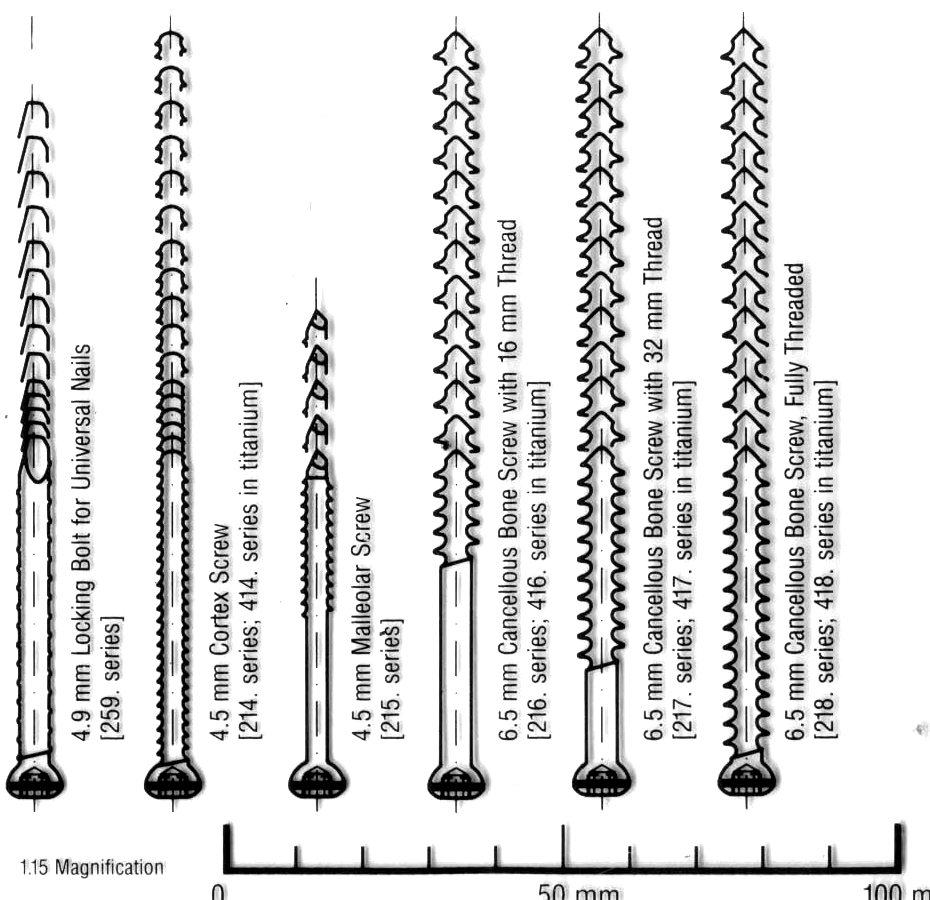
\includegraphics[width=.4\columnwidth]{images/plantillas.png}
	\caption{Un ejemplo de una plantilla (\textit{template}) de tornillos utilizados en una planificaci\'on}
	\label{fig:plantilla}
\end{figure}

Las plantillas (\textit{templates}) son implantes bases construidos por un fabricante bajo diversos materiales y con diferentes medidas. Los implantes que se muestran en las plantillas, sirven de gu\'ia exacta al momento de realizar una reducci\'on y fijaci\'on interna para un paciente. El almacenamiento de estas plantillas se realiza de forma manual bajo criterio propio del Departamento de Radiolog\'ia. Al momento de utilizar una plantilla, es importante conocer la categor\'ia de la fractura as\'i como un diagn\'ostico previo con el fin de determinar su utilizaci\'on \'o no.

Es importante destacar que para la realizaci\'on manual de una reducci\'on de fractura se requiere una inversi\'on de tiempo. Si la inversi\'on de tiempo fuese menor para cada caso de fractura que requiera cirug\'ia, entonces los costos del centro hospitalario se reducen de forma considerable ya que se obtiene mayor tiempo productivo de los m\'edicos cirujanos.

%%%%%%%%%%%%%%%%%%%%%%%%%%%%%%%%%%%%%%%
\subsection{Antecedentes de sistemas CAOS}

Al momento de una cirug\'ia, la elecci\'on del procedimiento quir\'urgico viene determinado por las caracter\'isticas de la fractura u osteotom\'ia: hueso, regi\'on, tipo de trazo, desviaciones angulares, rotaciones, acortamientos, n\'umero de fragmentos, tama\~no de los fragmentos y las condiciones de los tejidos blandos. Dada la cantidad de factores a considerar para dicho procedimiento, R\"{u}edi et al. \cite{website:ruedi} sugieren la creaci\'on de un plan para la cirug\'ia que incluya todos los pasos a realizar de forma ordenada durante el acto quir\'urgico. 

La literatura relacionada con sistemas CAD para fracturas es poca, pero existen trabajos relevantes centrados en la detecci\'on de osteoporosis  y estimaci\'on de la edad de huesos. Uno de los trabajos de mayor aporte en el \'area de detecci\'on de fracturas en huesos largos fue el realizado por Tian et al. \cite{TIAN03} en el 2003, los cuales desarrollaron un algoritmo para detectar las fracturas en el f\'emur y el radio. 

El m\'etodo descrito por Tian et al. \cite{TIAN03} detecta una fractura en el f\'emur solamente en el cuello del mismo. Su t\'ecnica calcula el \'angulo entre el eje del cuello del f\'emur y el eje del f\'emur, llamado \'angulo NSA (\'Angulo del Cervico Diafisiario - \textit{Neck-Shaft Angle}), y trabaja sobre im\'agenes de CT en formato DICOM. Esta medida del \'angulo es realizada en tres etapas: la primera etapa consiste en la extracci\'on del contorno del f\'emur, ver Figura \ref{fig:tian}, la segunda etapa se refiere al c\'alculo del \'angulo NSA, y la tercera es la clasificaci\'on del \'angulo obtenido. La extracci\'on del contorno del f\'emur descrita por Tian et al. \cite{TIAN03}, utiliza la detecci\'on de bordes propuesta por Canny \cite{CANNY86}, la transformada de Hough \cite{DUDA72} y un modelo de Contornos Activos \cite{KASS88}.
\begin{figure}[htb]
	\centering
	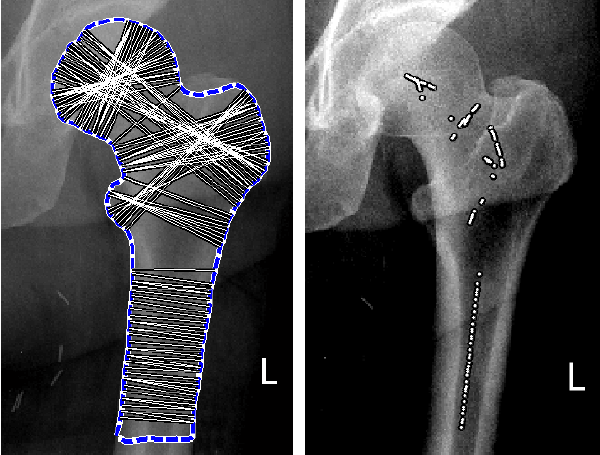
\includegraphics[width=.5\columnwidth]{images/tian.png}
	\caption{L\'ineas encontradas en la detecci\'on del contorno del fem\'ur y l\'ineas gu\'ias para determinar la l\'inea central del fem\'ur. Imagen extra\'ida de \cite{TIAN03}}
	\label{fig:tian}
\end{figure}

En el a\~no 2004 Yap et al. \cite{YAP04} mejoran el m\'etodo aplicado por Tian et al. \cite {TIAN03} para la detecci\'on de fracturas en el f\'emur. Ellos trabajan igualmente sobre im\'agenes de CT, incluyendo el an\'alisis de la perturbaci\'on de los patrones presentes en la trabecular del cuello femoral. De la misma forma, su m\'etodo consiste en 3 etapas: 
\begin{enumerate}
	\item La extracci\'on del contorno del f\'emur.
	\item El an\'alisis de la textura trabecular.
	\item Clasificaci\'on de la fractura.
\end{enumerate}

Para la extracci\'on del f\'emur en la imagen utilizaron un Modelo de Contornos Activo (\textit{snake}) con flujo del vector gradiente. Los resultados obtenidos en este trabajo arrojaron un 84.6\% de exactitud en la detecci\'on de fracturas.

Los m\'etodos mencionados anteriormente producen resultados aceptables, pero tienen como desventaja que solamente trabajan en fracturas localizadas en el cuello femoral y no pueden ser adaptados para otros huesos. Otro factor desfavorable con respecto a estos m\'etodos es originado por el uso de Contornos Activos, porque est\'a t\'ecnica requiere que el m\'edico coloque los puntos iniciales del Contorno Activo y ajuste el modelo la cantidad de veces que sea necesario hasta lograr los resultados esperados.

Una mejora a estos m\'etodos fue introducida por Lim et al. \cite{LIM04} en el 2004, donde se modifica el algoritmo de extracci\'on del contorno propuesto por Tian et al. \cite{TIAN03} incluyendo Campos Aleatorios de Markov (\textit{MRF - Markov Random Fields}) e intensidad en la direcci\'on del gradiente (\textit{IGD - Intensity Gradient Direction}) al m\'etodo existente del NSA y tambi\'en incluyendo mapas de orientaci\'on Gabor (\textit{GO - Gabor Orientation}) \cite{AKDE05}. Adem\'as, Lim et al. \cite{LIM04} modificaron la clasificaci\'on planteada en \cite{YAP04}, y consiguieron una detecci\'on de fracturas del 92.2\% de exactitud y 1\% de detecci\'on de fracturas cuando en realidad no exist\'ian (falso positivo). Un ejemplo de la detecci\'on de fracturas se puede observar en la Figura \ref{fig:lim}.
\begin{figure}[htb]
	\centering
	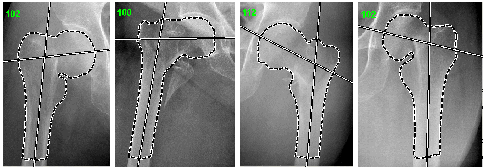
\includegraphics[width=.75\columnwidth]{images/fracturedfemur.png}
	\caption{Identificaci\'on de fracturas en el f\'emur, extra\'ido de Lim et al. \cite{LIM04}}
	\label{fig:lim}
\end{figure}

Los m\'etodos explicados anteriormente trabajan con im\'agenes CT en formato DICOM obtenidas directamente desde los equipos radiol\'ogicos. Este aspecto resulta una ventaja ya que la adquisici\'on de las im\'agenes se realiza en un solo paso, empleando la arquitectura existente (e.g. un PACS - \textit{Picture Archiving and Communication System}) en el centro hospitalario.

Al resultar la segmentaci\'on de huesos un aspecto muy ligado a la anatom\'ia del mismo, existen m\'etodos de clasificaci\'on que eval\'uan las caracter\'isticas de la imagen de una fractura y la ubica en un tipo de fractura. Uno de \'estos es el m\'etodo planteado por Su et al. \cite{SU99} el cual utiliza una red neuronal como sistema clasificatorio de fracturas.

Los sistemas CAD de planificaci\'on preoperatoria para fracturas fueron surgiendo como una opci\'on donde la segmentaci\'on de los fragmentos de la fractura, es autom\'atica, semiautom\'atica o manual.  La segmentaci\'on autom\'atica tiene buenos resultados para fracturas conocidas sobre partes espec\'ificas de la anatom\'ia (e.g. cadera, h\'umero, etc.), pero no funciona correctamente si se le aplica a una hueso arbitrario, por lo que no se puede considerar como la \'unica opci\'on. Por su parte, la segmentaci\'on semiautom\'atica genera una segmentaci\'on inicial que sirve de gu\'ia y as\'i el m\'edico puede ir mejor\'andola con su intervenci\'on. La segmentaci\'on manual, deja completamente esta tarea a cargo del m\'edico que est\'a realizando la planificaci\'on.

En el 2001, Mihalko et al. \cite{MIHA01} presentan un sistema CAD que permite medir la longitud del hueso antes y despu\'es de la colocaci\'on de un implante y de esta forma poder medir la deformaci\'on del mismo, siendo una herramienta preoperatoria y postoperatoria de una fractura.  En el 2002, Viceconti et al. \cite{VICE03} presentan un sistema de planificaci\'on preoperatoria para el reemplazo total de cadera donde se utilizan radiograf\'ias convencionales, lo que le permite ser aplicado a una amplia gama de casos de pacientes de un Centro Hospitalario. 

Gran parte de las aplicaciones CAOS comerciales trabajan las planificaciones sobre im\'agenes en formato DICOM obtenidas de tom\'ografos, equipos de rayos-X, entre otros. Esto se debe a que ofrecen una soluci\'on integral como parte del PACS instalado en un centro hospitalario. Al tener radiograf\'ias convencionales, obtenidas con equipos no digitales, es necesario digitalizar dichas placas radiogr\'aficas.

Basado en la idea de digitalizar placas radiogr\'aficas convencionales, salieron al mercado diversos sistemas CAOS comerciales como NovaRAD \cite{REF_NOVA}, TraumaCAD \cite{REF_TRAUMA} y Sectra OrthoStation Package \cite{REF_SECTRA}, los cuales permiten realizar la planificaci\'on preoperatoria de forma digital (realizando digitalizaci\'on de las im\'agenes) y ofrecen una librer\'ia de implantes comerciales a utilizar entre muchas de sus funciones. En la Figura \ref{fig:trauma_cads}, se muestra un ejemplo de colocaci\'on de un implante (color verde) en una planificaci\'on empleando TraumaCAD \cite{REF_TRAUMA}.
\begin{figure}[ht]
	\centering
	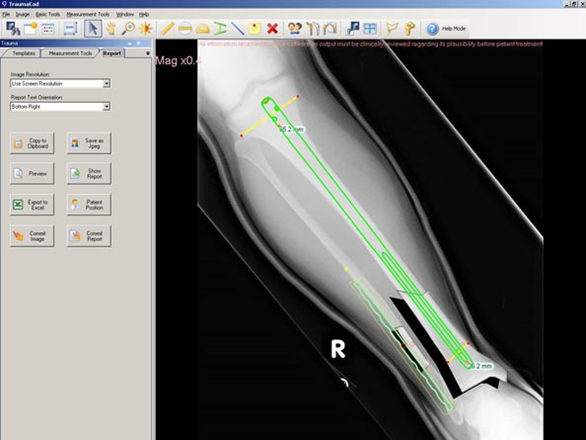
\includegraphics[width=.55\columnwidth]{images/trauma_cads.png}
	\caption{Colocaci\'on de un implante dentro de la aplicaci\'on TraumaCAD de OrthoCrat Ltd. \cite{REF_TRAUMA}}
	\label{fig:trauma_cads}
\end{figure}

En muchas ocasiones, es necesario moldear el implante tal que sea anat\'omicamente correcto y se adapte a una secci\'on del cuerpo. Este moldeado del implante consiste en un doblado que se realiza durante la operaci\'on, dentro del quir\'ofano. El doblado se aplica empleando una fuerza mec\'anica con una pinza especial. Cabe destacar que dichos sistemas no aplican deformaciones a sus plantillas ya que son est\'aticas, presentadas como un repositorio de im\'agenes.

En el siguiente cap\'itulo, se presenta un esquema general para los sistemas CAOS en la realizaci\'on de la planificaci\'on preoperatoria digital, incluyendo funcionalidades adicionales no existentes dentro de los sistemas mencionados anteriormente.